\documentclass[11pt]{exam}
\usepackage[margin=1in]{geometry}
\pagestyle{plain}
\usepackage{amsmath,amsfonts,amssymb,amsthm,enumerate}
\usepackage{multicol}
\usepackage[]{graphicx}
\usepackage{hyperref}
\usepackage{tikz}
\usepackage{pgfplots}
\usepackage{subfigure}
\usepackage[final]{pdfpages}

\addtolength{\footskip}{2\baselineskip} % to lower the page numbers
\title{\vspace{-0.5in} Math 115 \\ Worksheet Section 4.2}
\date{}


% \theoremstyle{definition}
% \newtheorem{problem}{Problem}
\renewcommand{\questionlabel}{\textbf{Problem~\thequestion.}}
% \printanswers

\begin{document}
\maketitle
\vspace{-0.75in}
A point $p$ in the domain of $f$ is a \textbf{global maximum} of $f$ on a given interval if $f(p)\geq f(x)$ for all $x$ in the interval.  
\vskip2ex
A point $p$ in the domain of $f$ is a \textbf{global minimum} of $f$ on a given interval if $f(p)\leq f(x)$ for all $x$ in the interval.  
\begin{questions}
  \question For each of the following graphs, locate any global maxima or minima on the interval drawn, if they exist.

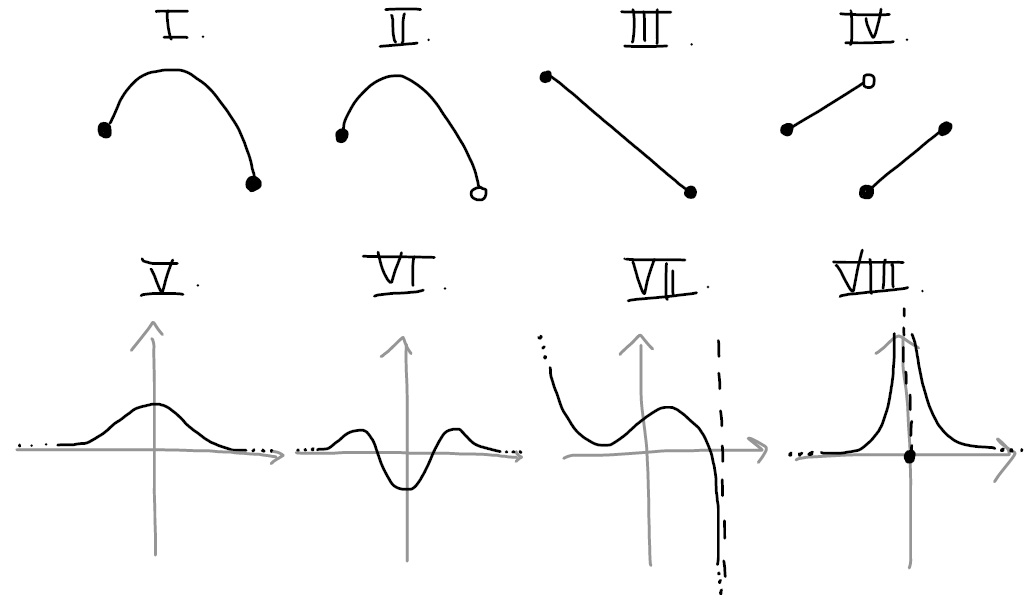
\includegraphics[width=6in]{graphs.jpg}
\begin{solution}
  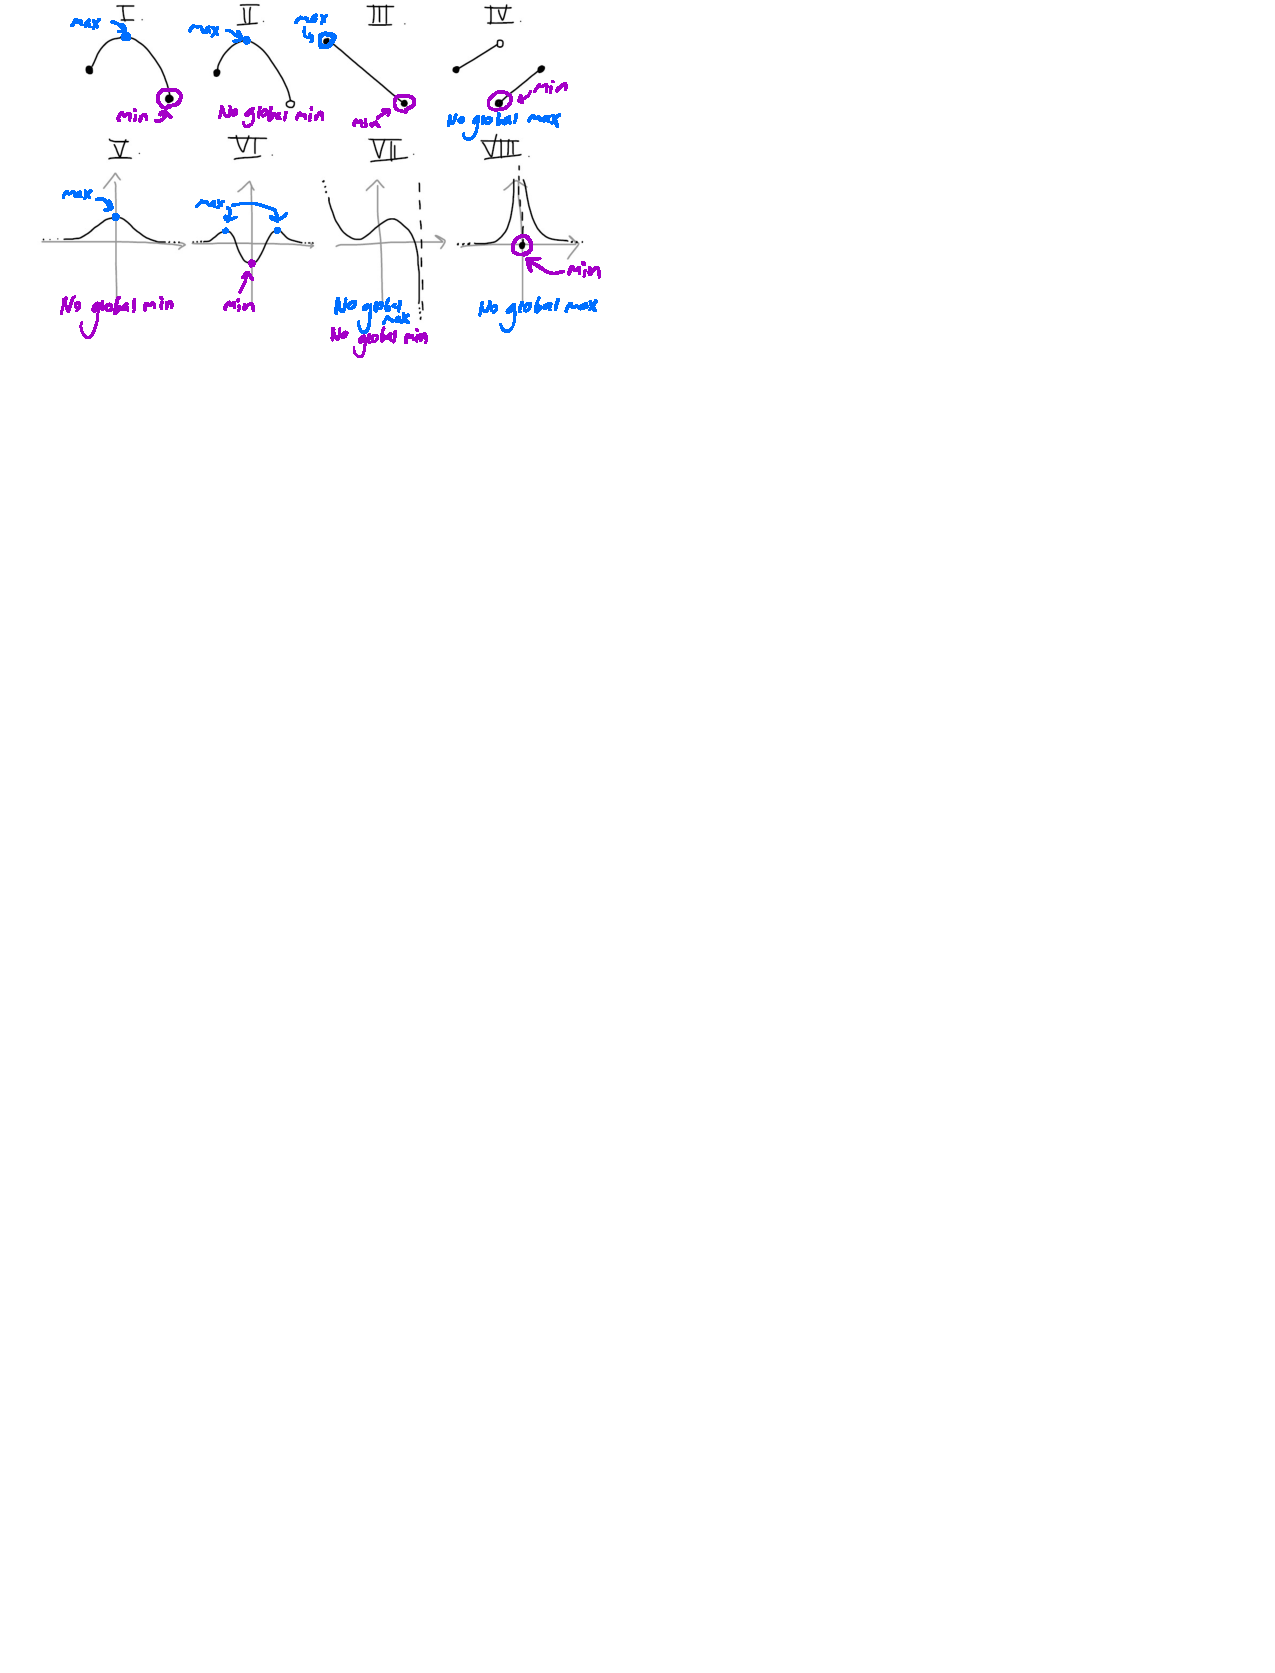
\includegraphics[]{4.2-graphs}
\end{solution}
\question Let $g(x) = x^3e^{-x}$.
\begin{enumerate}[(a)]
\item Find any global minima and maxima of $g$ on $(1,\infty)$.
\vfill
\item Now find any global minima and maxima of $g$ on $[0,\infty)$.
\vfill
\item Now find any global minima and maxima of $g$ on $(-\infty,\infty)$.
\end{enumerate}
\begin{solution}
  For all the parts, we will need \(g'(x) = 3x^2 e^{-x} - x^3 e^{-x} =
  x^2(3-x)e^{-x}\). We also compute
  \begin{itemize}
  \item \(g'(x) = 0\): at \(x=0,3\)
  \item \(g'(x)\) DNE: none
  \end{itemize}
  \begin{enumerate}[(a)]
  \item On \((1,\infty)\), the only critical value to consider is
    \(x=3\). However, we must also consider the end behavior for \(x
    \to 1^+\) and \(x \to \infty\).
    \begin{itemize}
    \item \(\lim_{x \to 1^+} g(x) = 1^3 e^{-1} = \frac{1}{e}\)
    \item \(g(3) = 3^3 e^{-3} = \frac{27}{e}\)
    \item \(\lim_{x \to \infty} g(x) = 0\) since \(e^{-x}\) dominates
      \(x^3\). 
    \end{itemize}
    Alternatively, we can check that the one critical point \(x=3\) is
    a local maximum and, since it is the only one, it must also be a
    global maximum: \\

    \begin{tikzpicture}
      \node at (-1,0) {$g'$};
      \draw (0,0)--(4,0);
      \draw (2,-.1)--(2,.1);
      \node at (2,-.4) {$3$};
      \node at (1,.2) {$+\cdot + = +$};
      \node at (3,.2) {$- \cdot + = -$};
      \node at (0,0) {$\big($};
      \node at (0,-.4) {$1$};
    \end{tikzpicture}

    So, \(g\) has a global maximum at \(x=3\) and no global minimum on
    the interval \((1,\infty)\).
  \item On \([0,\infty)\), we now must consider \(g(0)\), since it is
    an endpoint (it is also a critical point).
    \begin{itemize}
    \item \(g(0) = 0 \cdot 1 = 0\)
    \item \(g(3) = \frac{27}{e}\)
    \item \(\lim_{x \to \infty} g(x) = 0\)
    \end{itemize}
    So, by similar reasoning to the above, \(g(x)\) has a global
    maximum at \(x=3\) on \([0,\infty)\). However, \(g(x)\) also achieves a global
    minimum at \(x=0\) since \(g\) never goes below \(0\) on \([0,\infty)\).
  \item On \((-\infty,\infty)\), we must consider all the critical
    points and the end behavior 
    \begin{itemize}
    \item \(\lim_{x \to -\infty} x^3 e^{-x} = -\infty\) (DNE)
    \item \(g(0) = 0\)
    \item \(g(3) = \frac{27}{e}\)
    \item \(\lim_{x \to \infty} x^3 e^{-x} = 0\).
    \end{itemize}
    Thus, on \((-\infty,\infty)\), \(g(x)\) has a global maximum at
    \(x=3\) by the same reasoning as above. However, on
    \((-\infty,\infty)\), \(g(x)\) has no global minimum since the
    limit as \(x \to -\infty\) is \(-\infty\).
  \end{enumerate}
\end{solution}
\question Find any global extrema of the following function on its domain.
$$h(x) = \left\{
\begin{array}{ll}
      2e^{x-1}& 0\leq x\leq 1 \\
      (x-3)^2-2 & 1<x\leq 4 
\end{array} 
\right.
$$
\begin{solution}
  First, we observe that \(h(x)\) is, in fact, continuous at
  \(x=1\). However, \(h(x)\) is not differentiable at \(x=1\) since, for \[
    h'(x) =
    \begin{cases}
      2e^{x-1} & 0 < x < 1\\
      2(x-3) & 1 < x < 4
    \end{cases}
  \]
  the two pieces do not agree at \(x=1\). Thus, 
  \begin{itemize}
  \item \(h'(x) = 0\): \(x=3\)
  \item \(h'(x)\) DNE: \(x=1\) since \(2e^{1-1} = 2 \neq -4 = 2(1-3)\).
  \end{itemize}
  Since \(h(x)\) is continuous
  on \([0,4]\), we know \(h(x)\) has a global maximum and a global
  minimum by the \textbf{Extreme Value Theorem}. Furthermore, they
  must come from the critical points or the endpoints. We check
  \begin{itemize}
  \item \(h(0) = \frac{2}{e}\)
  \item \(h(1) = 2\)
  \item \(h(3) = -2\)
  \item \(h(4) = -1\)
  \end{itemize}
  Thus, \(h\) has a global maximum at \(x=1\) on \([0,4]\) and a
  global minimum at \(x=3\) on \([0,4]\).
\end{solution}
\question (Winter 2018 Exam 2) %problem 7
The amount of chlorine in a chemical reaction \(C(t)\) (in gallons) \(t\) seconds after it has been added into a solution is given by the function
$$C(t)=2-3(t-5)^{\frac{4}{5}}(t-1)e^{-t} \qquad \textrm{for } t \geqslant 0.$$
Notice that
$$C'(t)=\frac{3(t-6)(5t-9)e^{-t}}{5(t-5)^{\frac{1}{5}}} \qquad \textrm{for } t \geqslant 0.$$
\begin{enumerate}[(a)]
\item Use calculus to find the time(s) (if any) at which the amount of chlorine in the solution is the greatest and the smallest. 
\end{enumerate}
\begin{solution}
  See \href{https://dhsp.math.lsa.umich.edu/exams/115exam2/w18/s7.pdf}{https://dhsp.math.lsa.umich.edu/exams/115exam2/w18/s7.pdf}
\end{solution}
\question (Fall 2017 Exam 2) % problem 5
  Blizzard the snowman and his mouse friend Gabe arrived in Montana, where it has recently snowed. Since Blizzard is still melting, they decide to use this time to pack extra snow onto Blizzard, to help him make it to the North Pole. Let $H(t)$ be Blizzard's height, in inches, if Blizzard and Gabe stay in Montana for $t$ hours. On the interval $1 \leqslant t < \infty$, the function $H(t)$ can be modeled by
$$H(t) = 35 + 10 e^{-\frac{t}{6}}(t-2)^{\frac{1}{3}}.$$
Notice that
$$H'(t) = \frac{-5e^{-\frac{t}{6}}(t-4)}{(t-2)^{\frac{1}{3}}}.$$
\begin{enumerate}[(a)]
\item Find all values of $t$ that give global extrema of the function $H(t)$ on the interval $1 \leqslant t < \infty$. Use calculus to find your answers, and be sure to show enough evidence that the point(s) you find are indeed global extrema. For each answer, write none if appropriate.
\item Assuming Blizzard stays in Montana for at least 1 hour, what is the tallest height Blizzard can reach? Remember to include units.
\end{enumerate}
\begin{solution}
  See \href{https://dhsp.math.lsa.umich.edu/exams/115exam2/f17/s5.pdf}{https://dhsp.math.lsa.umich.edu/exams/115exam2/f17/s5.pdf}
\end{solution}
\question (Winter 2017 Exam 2) % problem 8
At Happy Hives Bee Farm, the population of bees, in thousands, $t$ months after the farm opens, can be modeled by $g(t)$, where
$$g(t) = \displaystyle\left\lbrace \begin{array}{ll} 20 + \displaystyle\frac{1}{3} e^{4-t} & \textrm{for } 0 \leqslant t \leqslant 4 \\  -\displaystyle\frac{1}{6}t^3  + \displaystyle\frac{9}{4} t^2 - 7 t + 23 & \textrm{for } 4 < t \leqslant 8 \end{array} \right.$$
and
$$g'(t) = \displaystyle\left\lbrace \begin{array}{ll} -\displaystyle\frac{1}{3} e^{4-t} & \textrm{for } 0 \leqslant t \leqslant 4 \\  -0.5(t-2)(t-7) & \textrm{for } 4 < t \leqslant 8 \end{array} \right.$$
\begin{enumerate}[(a)]
\item Find the values of $t$ that minimize and maximize $g(t)$ on the interval $[0, 8]$. Use calculus to find your answers, and be sure to show enough evidence that the points you find are indeed global extrema. For each answer, write none if appropriate.
\item What is the largest population of bees that occurs in the first
  8 months the farm is open?
\end{enumerate}
\begin{solution}
  See \href{https://dhsp.math.lsa.umich.edu/exams/115exam2/w17/s8.pdf}{https://dhsp.math.lsa.umich.edu/exams/115exam2/w17/s8.pdf}
\end{solution}
\pagebreak
\question (Fall 2017 Exam 2) % problem 6
  Sketch graphs of functions $f(x)$ and $g(x)$ satisfying the conditions below, or say that no such function exists. 
	\begin{enumerate}[(a)]
	\item A function $f(x)$ defined on the interval $(0,4)$ that satisfies 
	\begin{itemize}
	\item $f'(x) > 0$ for all $x \neq 2$, and
	\item $x=2$ is a global minimum.
	\end{itemize}
	\item A function $g(x)$ defined on the interval $(0,4)$ that satisfies 
	\begin{itemize}
	\item $\displaystyle\lim_{x \rightarrow 2^-} g'(x) = \infty$, and
	\item $\displaystyle\lim_{x \rightarrow 2^+} g'(x) = 0$.
	\end{itemize}
	\end{enumerate}
      \question (Winter 2017 Exam 2) % problem 7
        Sketch the graph of a single function $y = h(x)$ satisfying all the following:
\begin{itemize}
\item The function $h(x)$ is defined for $-7 \leqslant x \leqslant 7$.
\item $h(x)$ has global maximums at $x=-7$ and $x=3$.
\item $h(x)$ has an inflection point at $x = -5$.
\item $h(x)$ is continuous at $x = -3$ but not differentiable at $x = -3$.
\item $h(x)$ has a local minimum at $(-1, -4)$ but is not continuous at $x = -1$.
\item $h(x)$ has a critical point at $(2, 5)$ that is neither a local maximum or a local minimum.
\item $h(x)$ satisfies the conclusion of the Mean Value Theorem on $[4,7]$ but not the hypothesis of this theorem.
\end{itemize}
\begin{solution}
  See \href{https://dhsp.math.lsa.umich.edu/exams/115exam2/f17/s6.pdf}{https://dhsp.math.lsa.umich.edu/exams/115exam2/f17/s6.pdf}
\end{solution}
\question (Winter 2016 Exam 2) % problem 9
  Consider a continuous function \(T\) with the following properties.
  \begin{itemize}
  \item \(T(v)\) is defined for all real numbers v.
  \item The critical points
    of \(T(v)\) are the four points \(v = 3, v = 5, v = 7\), and \(v = 8\). (\(T(v)\)
    has no other critical points.)
  \end{itemize}
  Some values of \(T\) are shown in the following table:\\
  \begin{tabular}{|c|c|c|c|c|c|c|}
    \hline
    \(v\)&0&3&5&7&8&10\\
    \hline
    \(T(v)\)&21&9&13&19&11&21\\
    \hline
  \end{tabular}

  For each of a.-f. below, use the answer blank provided to list all the values \(v\) at which \(T(v)\) attains the specified global extremum. If there is not enough information provided to give an answer, write “not enough info”. If \(T(v)\) does not attain the specified global extremum on the specified interval, write “none”.

  For what value(s) \(v\) does \(T(v)\) attain its... 
  \begin{parts}
  \part global minimum on the interval \(0 \leq v \leq 10\)?
  \part global maximum on the interval \(0 \leq v \leq 10\)?
  \part global minimum on the interval \(0 < v \leq 10\)?
  \part global maximum on the interval \(0 < v \leq 10\)?
  \part global minimum on the interval \((-\infty,\infty)\)?
  \part global maximum on the interval \((-\infty,\infty)\)?
  \end{parts}
  \begin{solution}
    See \href{https://dhsp.math.lsa.umich.edu/exams/115exam2/w16/s9.pdf}{https://dhsp.math.lsa.umich.edu/exams/115exam2/w16/s9.pdf}
  \end{solution}
  \pagebreak
% \question Given that
% $$g(x) = 
%   \begin{cases}
%     \frac{2-x}{e}& x< 1 \\
%     x^2 e^{-x} & x \geq 1
%   \end{cases}
% $$
% \begin{enumerate}[(a)]
% \item Find any global extrema of $g(x)$ on the interval $[-4,2]$
% \item Find any global extrema of $g(x)$ on the interval $[1,\infty)$
% \end{enumerate}
\question (Winter 2016 Exam 2) % problem 6
Sketch the graph of a single function $y = g(x)$ satisfying all the following:
\begin{itemize}
\item $g(x)$ is defined for all x in the interval $-6 < x < 6$.
\item $g(x)$ has at least 5 critical points in the interval $-6 < x < 6$.
\item The global maximum value of $g(x)$ on the interval $-5 \leqslant x \leqslant -3$ is 4, and this occurs at $x = -4$.
\item $g(x)$ is not continuous at $x = -2$.
\item $g'(x)$ (the derivative of $g$) has a local maximum at $x = 0$.
\item $g(x)$ is continuous but not differentiable at $x = 1$.
\item $g''(x) \geqslant 0$ for all $x$ in the interval $2 < x < 4$.
\item $g(x)$ has at least one local minimum on the interval $4 < x < 6$ but does not have a global minimum on the interval $4 < x < 6$.
\item $g(x)$ has an inflection point at $x = 5$.
\end{itemize}
\begin{solution}
  See \href{https://dhsp.math.lsa.umich.edu/exams/115exam2/w16/s6.pdf}{https://dhsp.math.lsa.umich.edu/exams/115exam2/w16/s6.pdf}
\end{solution}
\end{questions}
\end{document}
%%% Local Variables:
%%% mode: latex
%%% TeX-master: t
%%% End:
